\documentclass[a4,12pt]{article}
\usepackage[utf8]{inputenc}
\usepackage[spanish]{babel}
\usepackage[margin=3cm]{geometry}
\usepackage{graphicx}
\usepackage{import}
\usepackage{color}
\usepackage{verbatim}
\usepackage{listings}
\usepackage[normalem]{ulem}
\usepackage{subfiles}
\usepackage{listingsutf8}
\usepackage{placeins}


\renewcommand{\familydefault}{\sfdefault}


\usepackage[hidelinks]{hyperref}

\newcommand{\grisclaro}{]{0.99}}
\newcommand{\gris}{\color[gray]{0.9}}
\newcommand{\grisos}{\color[gray]{0.5}}

\lstset{
	breaklines=true,
	breakatwhitespace=false,
	xleftmargin=1em,
	frame=single,
	numbers=left,
	numbersep=5pt,
}

\newcommand{\showprog}[3]
{
	
	\begin{minipage}{\textwidth}
		\lstinputlisting[language=python,
		frame=single,
		backgroundcolor=\gris,
		extendedchars=false,
		inputencoding=utf8/latin1,
		aboveskip=2eM,
		belowskip=2.5eM,
		basicstyle=\small,
		title=-- #1 --,
		columns=flexible,
		lastline=#2,
		firstnumber=#3,
		firstline=#3,
		commentstyle=\itshape\grisos,
		stringstyle=\color{blue}]
		{../src/#1}
	\end{minipage} 
}    
\begin{document}
	
	\subfile{portada.tex}
		
	
	
	\tableofcontents
	
		\begin{abstract}
			Esto es una pequeña comparación en Python entre tres algoritmos de búsqueda, en concreto, los siguientes:
			\begin{itemize}
				\item Ordenación por selección (mínimos sucesivos).
				\item Ordenación por inserción.
				\item Ordenación Timsort.
			\end{itemize}
		\end{abstract}
	
	\newpage
	
	\section{Introducción.}
	
	A continuación, vamos a comparar tres algoritmos de ordenación, entre ellos está el que usa \textbf{Python} (Timsort) en el método \textbf{sorted()} para ordenar listas, por ejemplo.\\
	
	Pediremos al usuario que introduzca un número, que será el tamaño de la lista a ordenar.\\
	
	\underline{La lista se rellenará automáticamente con números aleatorios}, y se usará la misma lista para los tres algoritmos.\\
	
	Finalmente, lanzaremos tres procesos en paralelo (uno con cada algoritmo de ordenación) y se compararán los tiempos de cada uno, y se mostrará por pantalla las listas ordenadas, junto con un gráfico comparativo de los tres algoritmos.\\
	
	Para llevar un control de las versiones del programa, y poder tener acceso al programa desde cualquier sitio, usaremos \textbf{Git} junto con \textbf{GitHub}.\\
	
	Además de esto, he trabajado con \textbf{Jupyter}, por lo que también se adjunta un fichero llamado Untitle.tex y Untitle.pdf con el código Python generado con Jupyter.
	
	%-- AQUI SE HABLA DE LOS ALGORITMOS UTILIZADOS...
	\section{Algoritmos utilizados.}
	En concreto, los algoritmos utilizados son siguientes:
	\begin{itemize}
		\item \textbf{Ordenación por selección} (mínimos sucesivos).
			\subitem El código está inspirado en el libro Python Fácil \cite{python_facil}. \\\\ $\bullet$ Es un doble bucle anidado, en el que se compara el primer número con todos los demás, y si alguno es menor, los intercambia de posición, luego se repite la misma operación con el segundo etcétera.
		\item \textbf{Ordenación por inserción}.
			\subitem El código está inspirado en el libro Python Fácil \cite{python_facil}. \\\\ $\bullet$ Este algoritmo, tiene un orden de ejecución de: $O(n^{2})$, además de ser inestable, es decir, puede que algún número no quede ordenado. Consiste en insertar un elemento de la lista en la parte $"$izquierda$"$ de la misma (los menores se desplazan a la izquierda), se repite este proceso desde el segundo hasta el último elemento de la lista.
		\item \textbf{Ordenación Timsort}.
			\subitem El código está implementado por los desarrolladores de Python \cite{manual}.\\\\ $\bullet$ Timsort es un algoritmo de clasificación estable (ordena siempre bien las listas) híbrido, derivado de la ordenación por ordenación y clasificación por inserción, diseñado para funcionar bien en muchos tipos de datos del mundo real
	\end{itemize}
	
	
	\section{Comparación de algoritmos}
	

	A continuación, se muestra una tabla comparativa con los tiempos de ejecución de los 3 algoritmos, con diferentes tamaños de lista. (tabla \ref{tab:tab1}):
	
	\begin{table}[h]
		\begin{center}
			
			\begin{tabular}{l|l|l|l|}
				Tamaño lista & Minimos sucesivos & Ordenacion por seleccion & Ordenacion por Timsort \\\hline
				200 & 0.002418 & 0.000693 & 0.000051 \\
				2000 & 0.190324 & 0.052366 & 0.000613 \\
				20000 & 14.562728 & 5.272498 & 0.005289
			\end{tabular}
			
		\end{center}
		
		\caption{Tabla con 2000 elementos}
		\label{tab:tab1}
	\end{table}
	Como podemos observar, vemos que, el que mejor se comporta para todos los tamaños es el algoritmo de ordenación Timsort, además, el algoritmo de ordenación por selección, ha fallado en la ordenación de 200 elementos, ya que ha dejado un número sin ordenar.\\
	
	También podemos observar, que, conforme crece el tamaño de la lista, el algoritmo que menos perjudicado se ve es el de Timsort, por ello se usa en la vida real para trabajar con grandes cantidades de datos de una forma eficiente.\\
	
	Los \textbf{ordenes de complejidad} de los algoritmos son los siguientes:
	\begin{itemize}
		\item Mínimos sucesivos
			\subitem $O(n^{2})$
		\item Ordenación por selección:
			\subitem $O(n^{2})$
		\item Ordenación por Timsort:
			\subitem $O(n\log{n})$
	\end{itemize}
	
	\section{Listados de código}
	A continuación, el código del programa, que está dividido en dos ficheros, uno con el módulo de los algoritmos y otro, con el programa principal.
	
	\showprog{program.py}{40}{0}
	\showprog{program.py}{75}{41}
	\showprog{program.py}{110}{76}
	
	\showprog{algoritmos\string_ordenacion.py}{35}{0}
	\showprog{algoritmos\string_ordenacion.py}{48}{36}
	
	\section{Flujo y entorno de trabajo.}
	Hemos utilizado las siguientes ramas en \textbf{Git}:
	
	\begin{itemize}
		\item Master $\mapsto$ Emula la rama maestra
		\item Develop $\mapsto$ Emula la rama de desarrollo
		\item Pro $\mapsto$ Emula la rama de producción
	\end{itemize}
	
	A continuación, se muestra los distintos cambios realizados en el repositorio, utilizando la herramienta \textbf{UpSource}.
			\begin{figure}[t]
				\begin{center}
					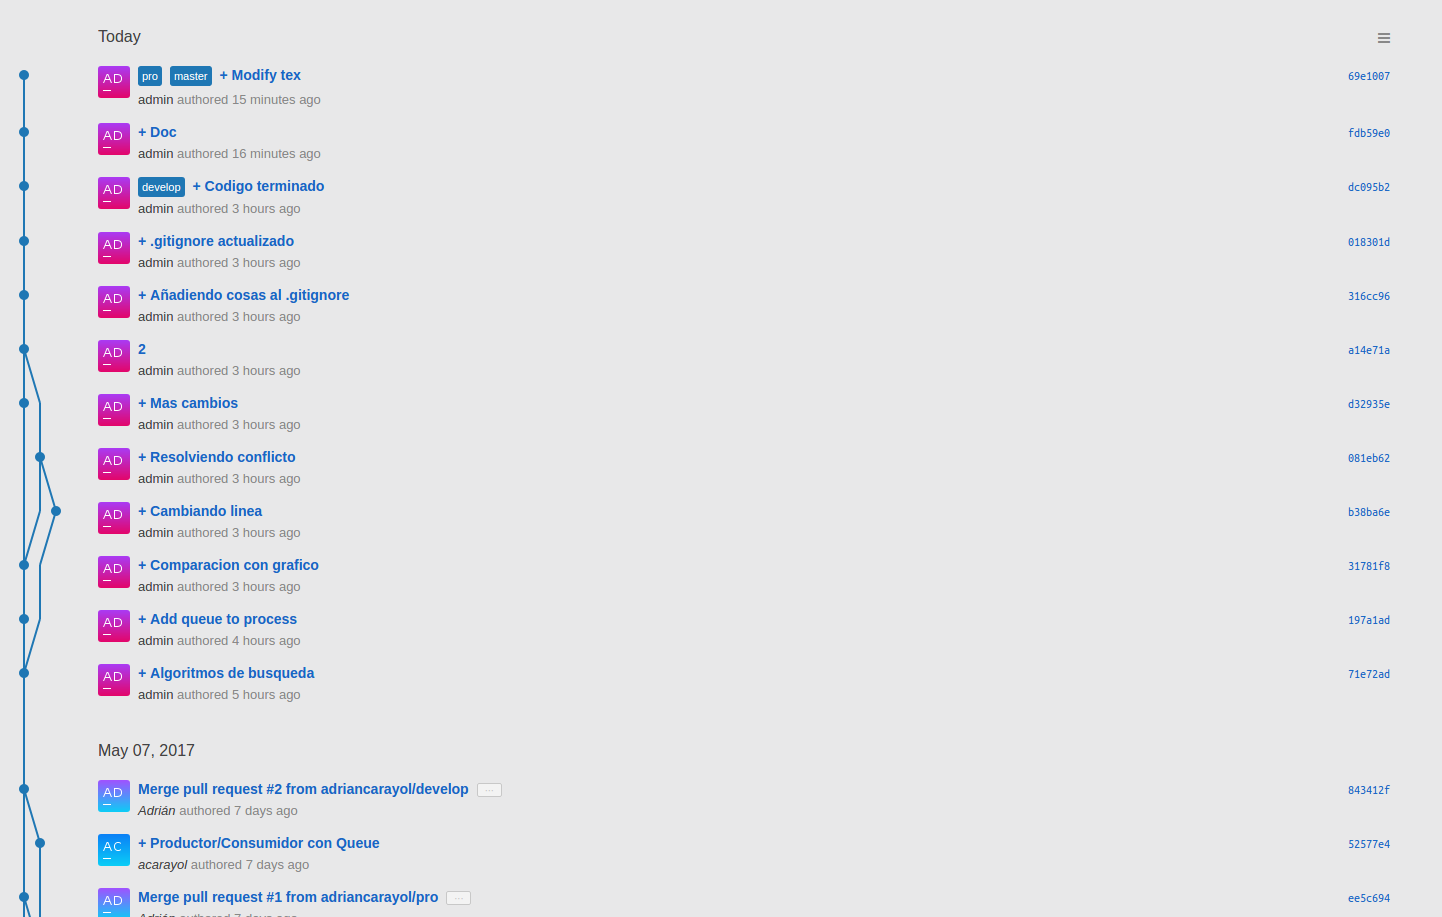
\includegraphics[scale=0.7, width=180mm]{pic3.png}
					\caption{Upsource para control del repositorio (1/2).}
				\end{center}
			\end{figure}
			\FloatBarrier
			
			
			\begin{figure}[t]
				\begin{center}
					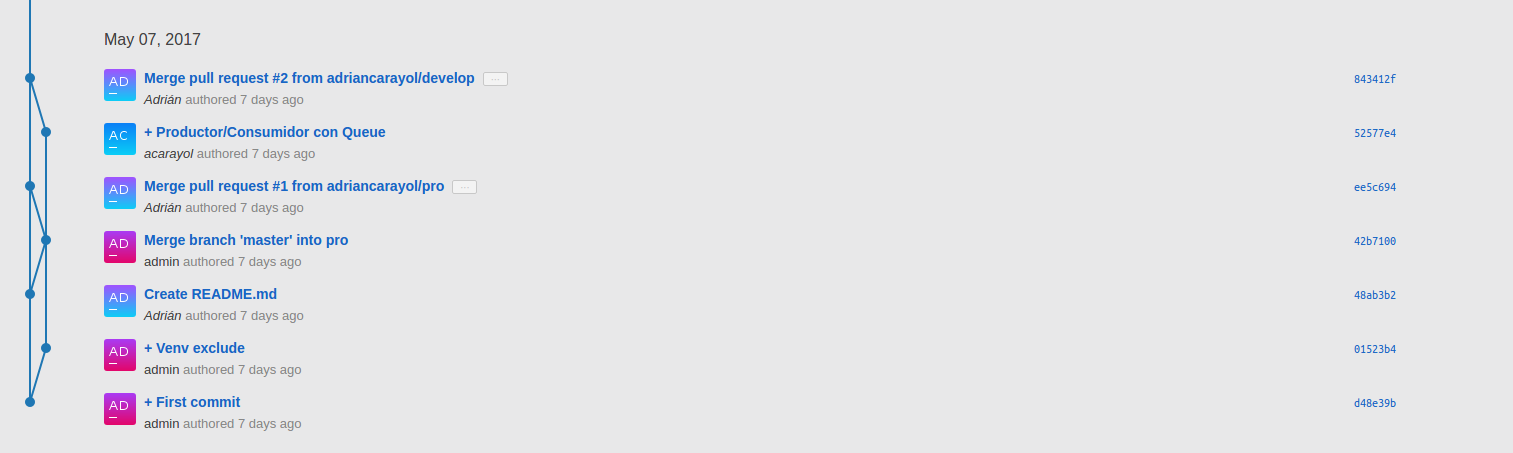
\includegraphics[scale=0.7, width=180mm]{pic4.png}
					\caption{Upsource para control del repositorio (2/2).}
				\end{center}
			\end{figure}
			\FloatBarrier
					
	Para el desarrollo del código en Python, he utilizado \href{https://www.jetbrains.com/pycharm/}{\colorbox{cyan}{PyCharm}}, que proporciona un entorno de desarrollo bastante completo, además, es de la misma compañía que UpSource.
	\section{Manual de uso.}
	
	
	%      itemize
	\begin{enumerate}
		\item Abrimos el terminal.
		
		\item Introducimos en el terminal el comando:
			\subitem \begin{verbatim} python3 program.py \end{verbatim}
		\item Indicamos el tamaño de la lista que queremos que ordene.
		\begin{figure}[t]
			\begin{center}
				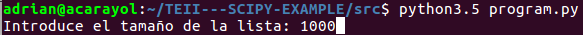
\includegraphics[scale=0.5]{pic1.png}
				\caption{Ejecución de programa.}
			\end{center}
		\end{figure}
		\FloatBarrier
		\item Esperamos a que el programa acabe.
		\item Se visualizará un gráfico con los tiempos comparativos de los 3 algoritmos, además de la lista ordenada por consola.
		\begin{figure}[t]
			\begin{center}
				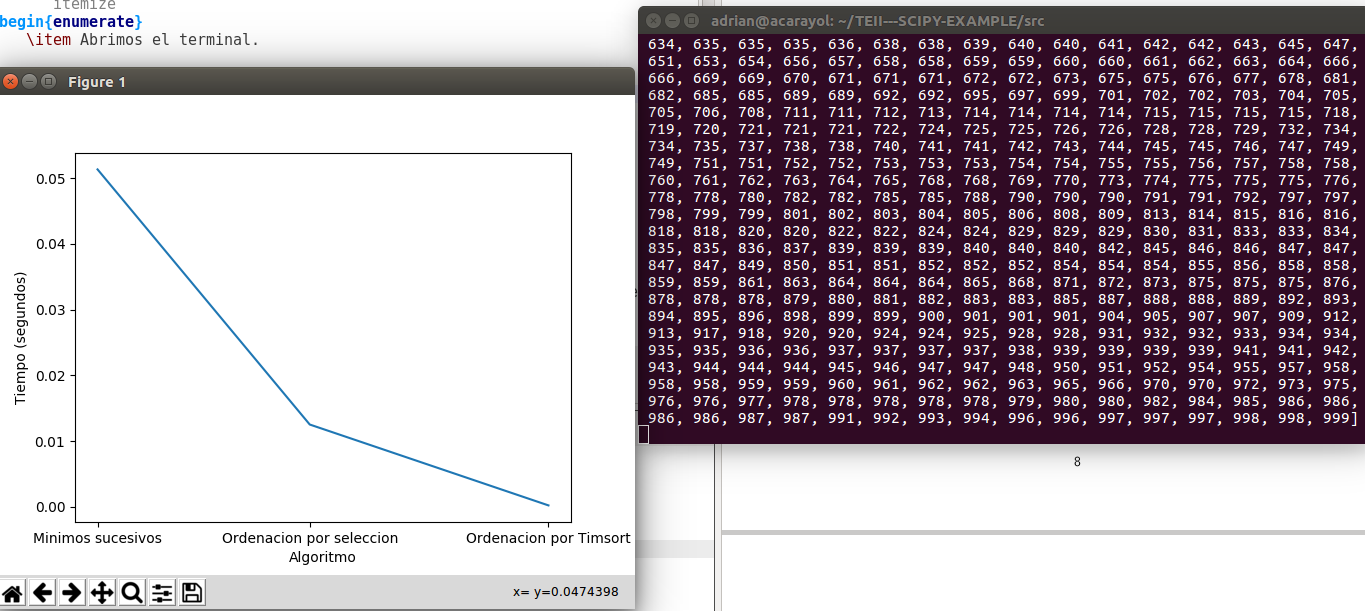
\includegraphics[scale=0.5]{pic2.png}
				\caption{Resultados de la ejecución.}
			\end{center}
		\end{figure}
		\FloatBarrier
		\item Cerramos el gráfico y el programa habrá finalizado.
	\end{enumerate}
	
	
	\section{Conclusión}
	
	El uso de \textbf{Latex} para preparar documentación es muy útil, ya que proporciona herramientas más completas y sofisticadas que las típicas herramientas de oficina.\\
	
	Respecto a \textbf{Git}, me parece una herramienta ideal para trabajar en equipo, remotamente, estés donde estés, y te permite poder realizar revisiones de todas las versiones que has subido a tu repositorio, por lo que te permite llevar un mayor control sobre todos los archivos.\\
	
	Finalmente, \textbf{Python}, me parece un lenguaje muy interesante y con una sintaxis sencilla, que, junto a sus cientos de módulos, te permite programar de una manera muy rápida.
	\clearpage
	
	\bibliographystyle{plain}  
	\bibliography{main-blx}
	
\end{document}











